\section{2d Web Symbols and Icons}


\begin{figure}
	\centering
	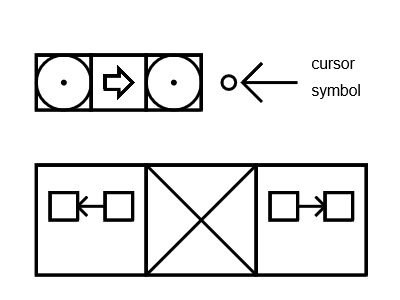
\includegraphics[width=3in]{figures/web2d/cursoredit.png}
	\caption[cursoredit]
	{cursor edits.}
\end{figure}

\begin{figure}
	\centering
	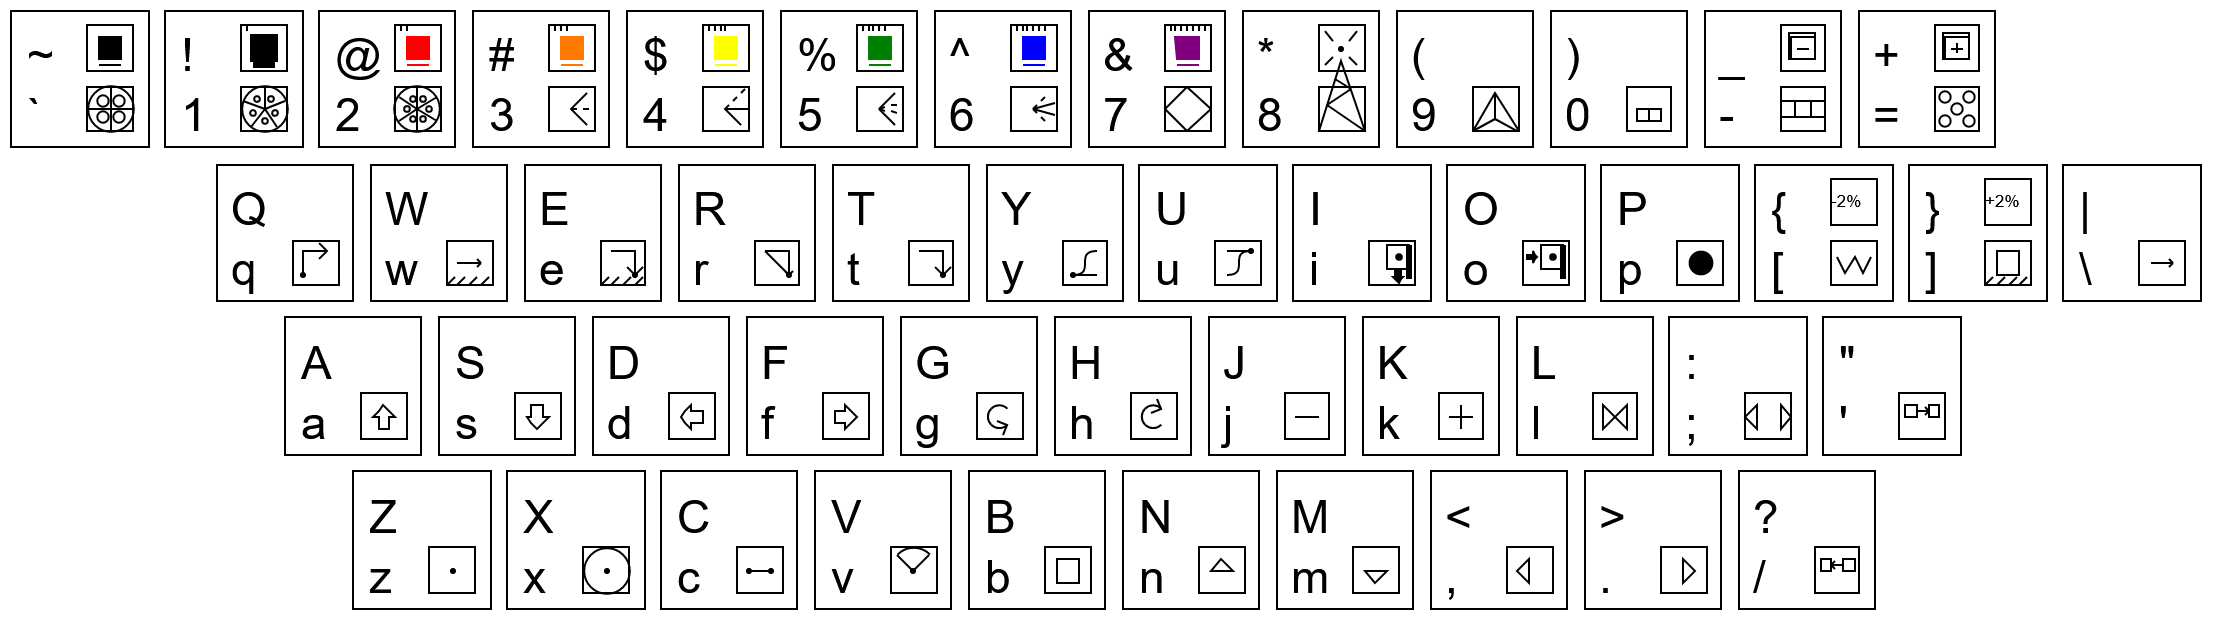
\includegraphics[width=4in]{figures/web2d/keyboard.png}
	\caption[keyboard]
	{keyboard.}
\end{figure}

\begin{figure}
	\centering
	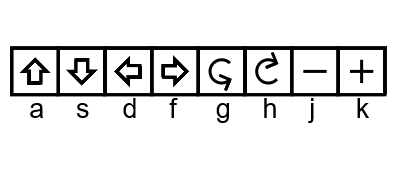
\includegraphics[width=4in]{figures/web2d/move.png}
	\caption[move]
	{Movements.  Arrows move along directions of the lines in the cursor.  Rotation is by the unit indicated by the cursor wing angles. Scale actions are by the current scale value as shown by the dot positions on the cursor.  Letters shown indicate the keys which map to these actions on a QWERTY keyboard with the default settings.}
\end{figure}

\begin{figure}
	\centering
	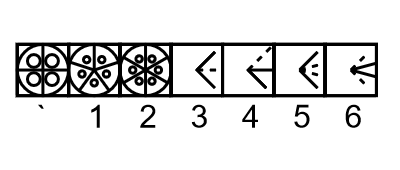
\includegraphics[width=4in]{figures/web2d/angles.png}
	\caption[angles]
	{Angles described by symmetry glyphs.  This also shows the actions to bisect, double, trisect and triple angles, and what keys are used to activate each geometric action.}
\end{figure}

\begin{figure}
	\centering
	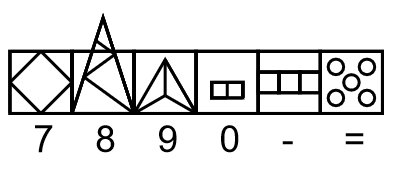
\includegraphics[width=4in]{figures/web2d/scaleactions.png}
	\caption[scaleactions]
	{Scales, along with keys used to map to them in default configuration. There is no relation between the numbers on the keys and the mathematics of the scales.  The scales shown are, from left to right, the square root of 2, the Golden Ratio, the square root of 3, 2, 3, and 5.}
\end{figure}

\begin{figure}
	\centering
	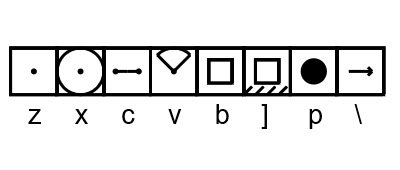
\includegraphics[width=4in]{figures/web2d/basicdraw.png}
	\caption[basicdraw]
	{Basic drawing actions, along with keys used in default configuration to activate them.  From left to right the actions are: draw dot, draw circle of unit radius, draw line segment of unit length, draw arc between cursor wings, draw a square, draw a filled square, draw a filled circle, and draw a line segment while moving forward one unit.}
\end{figure}

\begin{figure}
	\centering
	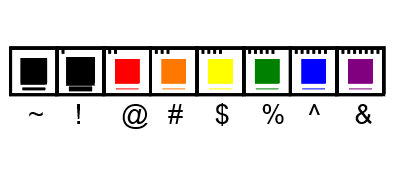
\includegraphics[width=4in]{figures/web2d/colors.png}
	\caption[colors]
	{Layers. Each layer has a line color, line width, and fill color, all of which are set with the Style object using the Style editor app.}
\end{figure}


\begin{figure}
	\centering
	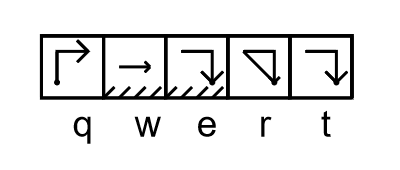
\includegraphics[width=4in]{figures/web2d/pathactions.png}
	\caption[pathactions]
	{Path actions, with keys used to activate them in default state.  From left to right, actions are: start path, draw line segment in path, close a filled path, close an unfilled path, and terminate a path without closing it.}
\end{figure}

\begin{figure}
	\centering
	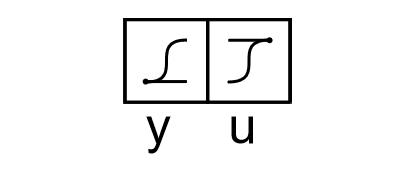
\includegraphics[width=4in]{figures/web2d/bezieractions.png}
	\caption[bezieractions]
	{Start a Bezier Path and terminate it with the y and u keys.}
\end{figure}


\begin{figure}
	\centering
	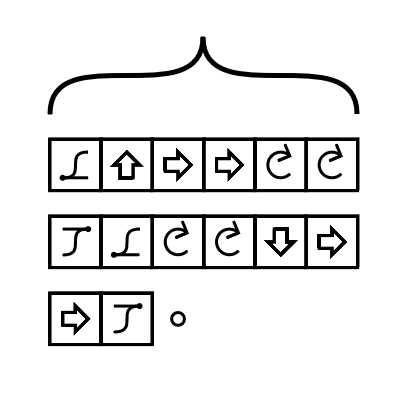
\includegraphics[width=4in]{figures/web2d/bezierbracket.png}
	\caption[bezierbracket]
	{Demonstrating the power of Geometron to make useful symbols with Bezier paths quickly and easily: a twiddle bracket.}
\end{figure}


\begin{figure}
	\centering
	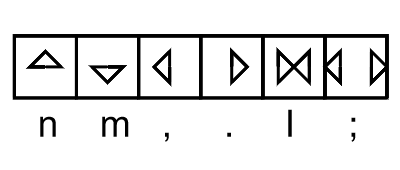
\includegraphics[width=4in]{figures/web2d/panzoom.png}
	\caption[panzoom]
	{Pan and zoom the field of view.}
\end{figure}

\begin{figure}
	\centering
	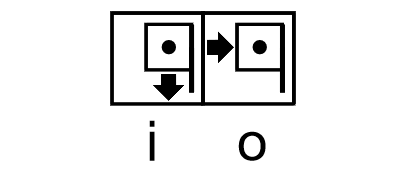
\includegraphics[width=4in]{figures/web2d/flagactions.png}
	\caption[flagactions]
	{Drop a flag, return to flag.}
\end{figure}


\begin{figure}
	\centering
	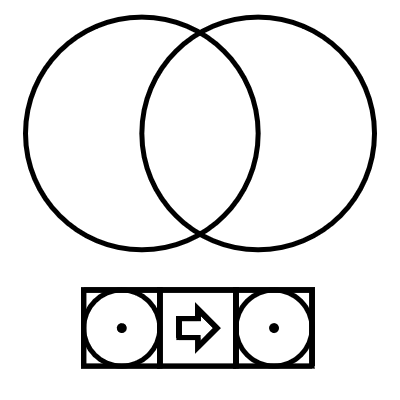
\includegraphics[width=4in]{figures/web2d/vesicapiscis.png}
	\caption[vesicapiscis]
	{The ``hello world'' of geometric programming, the Vesica Piscis.}
\end{figure}
\begin{figure}
	\centering
	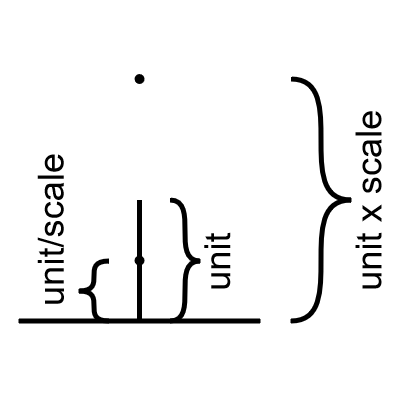
\includegraphics[width=4in]{figures/web2d/cursorscale1.png}
	\caption[cursorscale]
	{Cursor scale.}
\end{figure}
\begin{figure}
	\centering
	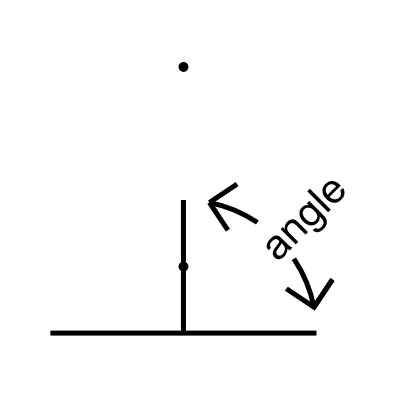
\includegraphics[width=4in]{figures/web2d/cursorangle1.png}
	\caption[cursorangle]
	{Cursor angle.}
\end{figure}
\begin{figure}
	\centering
	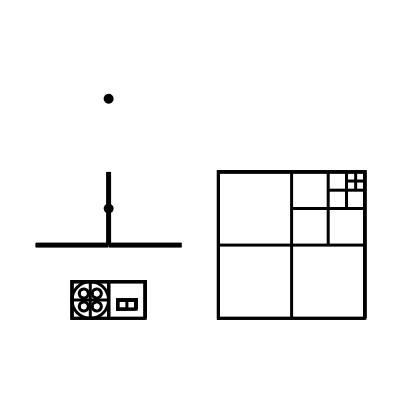
\includegraphics[width=4in]{figures/web2d/cursorsquare.png}
	\caption[cursorsquare]
	{Cursor square.}
\end{figure}
\begin{figure}
	\centering
	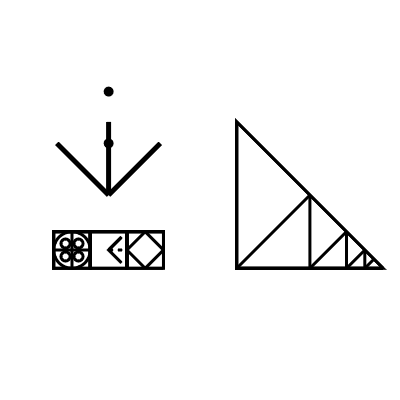
\includegraphics[width=4in]{figures/web2d/cursorroot2.png}
	\caption[cursorroot2]
	{Cursor root2.}
\end{figure}
\begin{figure}
	\centering
	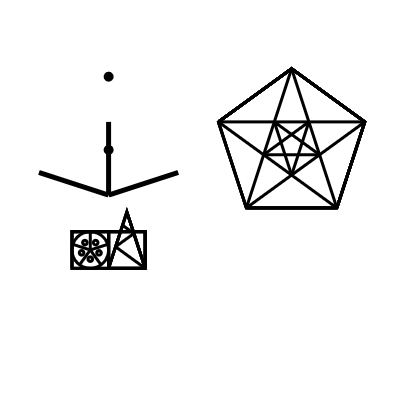
\includegraphics[width=4in]{figures/web2d/cursorgolden.png}
	\caption[cursorgolden]
	{Cursor golden ratio.}
\end{figure}
\begin{figure}
	\centering
	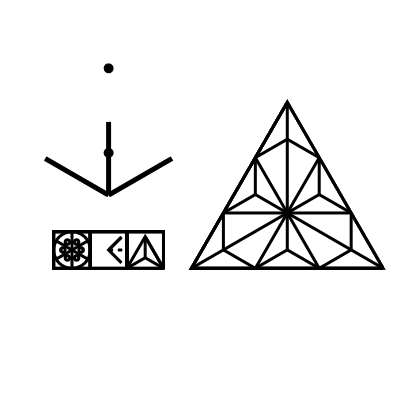
\includegraphics[width=4in]{figures/web2d/cursorroot3.png}
	\caption[cursorroot3]
	{Cursor root 3.}
\end{figure}
\begin{figure}
	\centering
	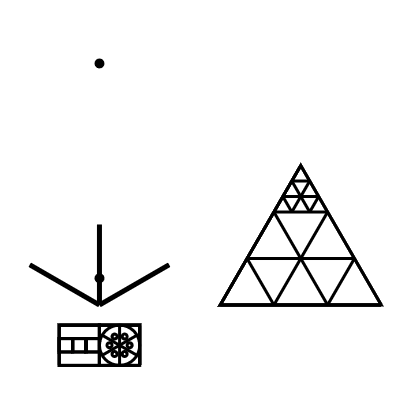
\includegraphics[width=4in]{figures/web2d/cursor3.png}
	\caption[cursor3]
	{Cursor 3.}
\end{figure}
\begin{figure}
	\centering
	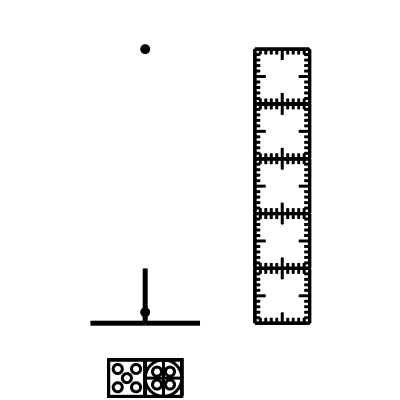
\includegraphics[width=4in]{figures/web2d/cursor5.png}
	\caption[cursor5]
	{Cursor 5.}
\end{figure}


\subsection{Style}

Each instance of the Geometron Virtual Machine has a style object, which defines 8 layers, numbered from 0 to 7.  Each style has a line color, line width, and fill color.  The properties of the style object are stored in the JSON file data/currentjson.txt which is used by the app symbol.html to edit graphics which are used by the rest of the Geometron system.  

\begin{figure}
	\centering
	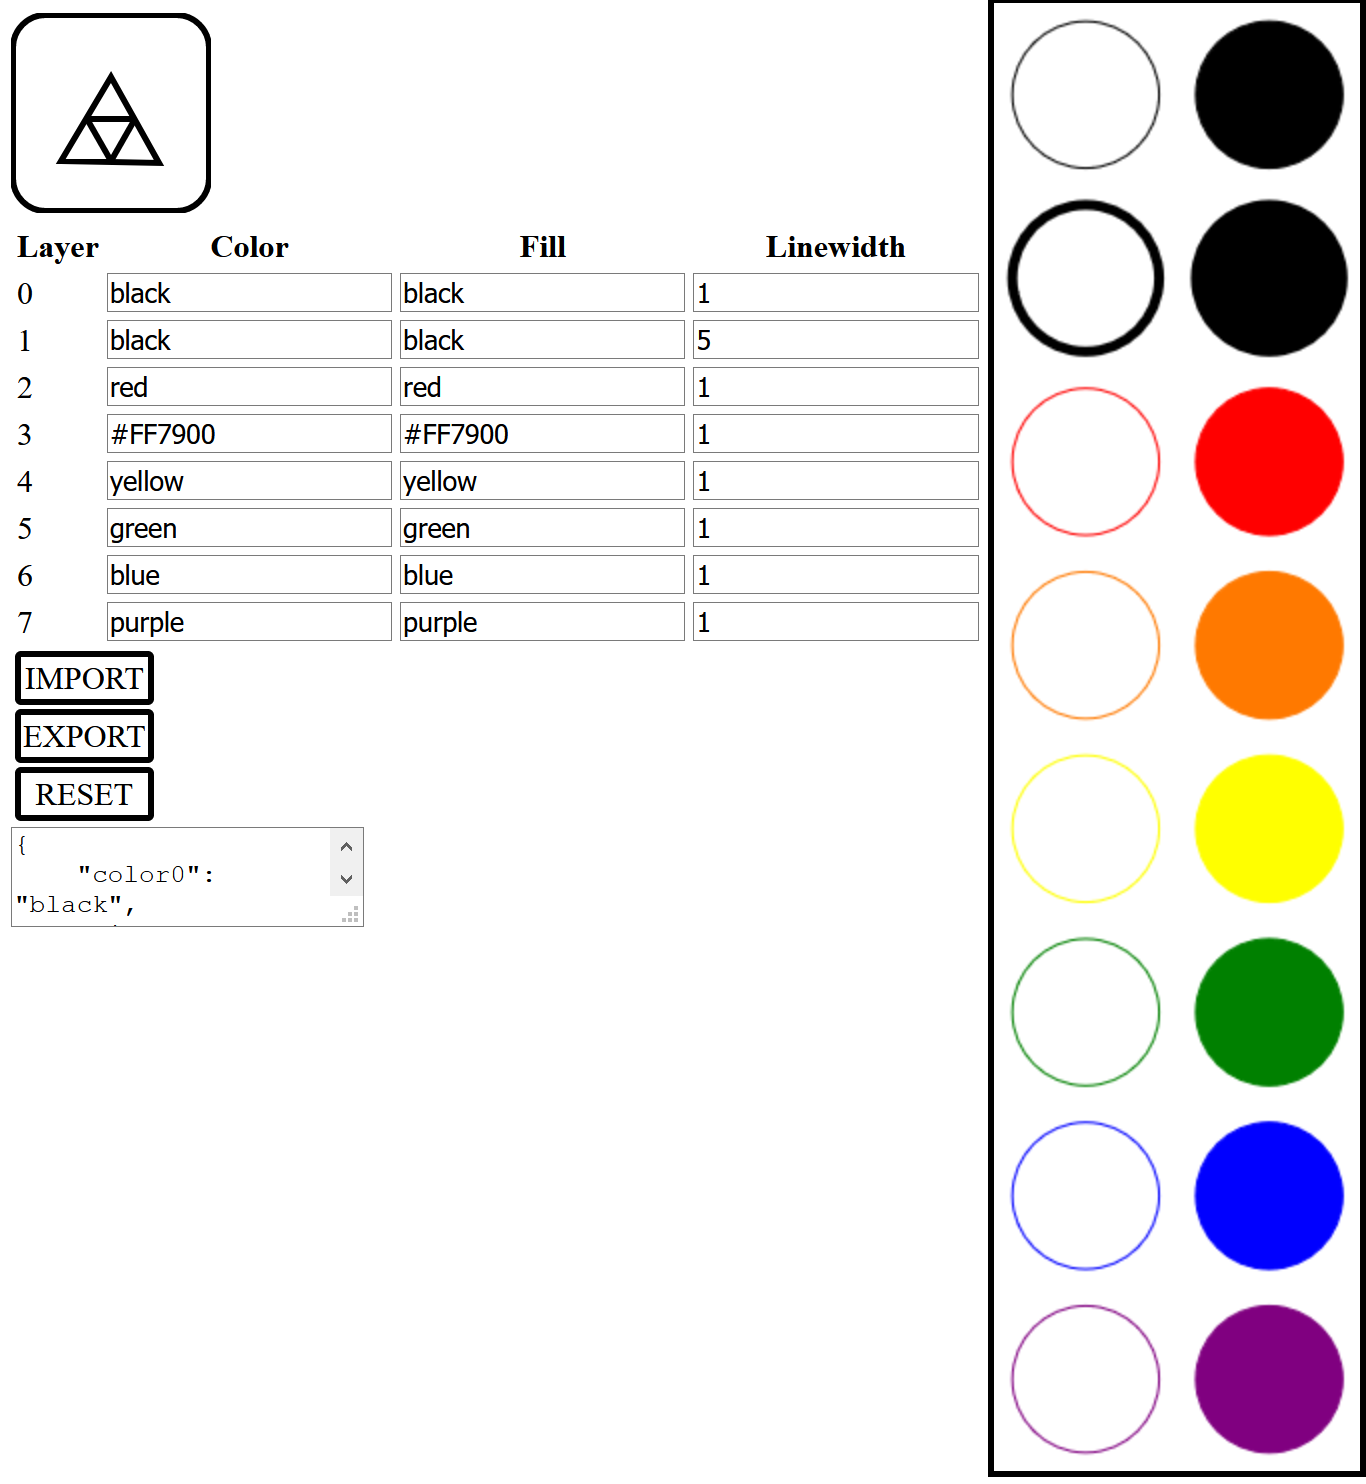
\includegraphics[width=4in]{figures/web2d/styleeditor.png}
	\caption[styleeditor]
	{Screen shot of the style editor app at styleeditor.html.  The display on the right hand side of the screen shows an unfilled circle and filled circle of each layer's style.  The text area in the bottom left of the screen is used to import and export style data, which can be saved offline and shared with other users via text message, email, etc.  The RESET button resets the style to a standard setting, which will erase any changes made to the existing style. Enter new values into any field to immediately change it.}
\end{figure}

While the style app edits the data file currentjson.txt which applies to the whole Geometron object used for symbol editing, the importing and exporting of data for sharing with other users only includes style information, without the rest of the JSON data.  This allows styles to be separated from the rest of the information for the purposes as usual of building a robust remix culture where Geometron users can constantly be sharing each piece of the system.  The EXPORT button will always post the current style JSON in the window in the lower left of the screen.  IMPORT will import the data, and RESET returns it to a default state.  Try creating your own new style with unusual line widths and colors, then exporting it and saving it offline, sharing it with other users, etc.  

Colors are in the format of HTML/CSS/JavaScript, and can be either names of colors like ``red'' or RGB color values like ``\#00ff00''.  This last format is a number in base 16 which has three 2 digit numbers in it(numbers between 0 and 0xFF), where the three numbers are values of red, green, and then blue.  So black is \#000000 and white is \#FFFFFF.  Any value where all three numbers are the same, like \#808080 will be a shade of grey.   Colors can be partially transparent by adding a fourth hexidecimal number which represents opacity.  So fully opaque red is \#FF0000FF, and red with half transparency is #FF000080(80 because 8 is half of 16, this is actually 128 in decimal).

\subsection{Graphics Setup}

The next section of the JSON we want to know how to edit in order to be able to make useful graphics is the setup, edited in the app setup.html.  Setup edits five numbers, all of which are in units of pixels: x0, y0, unit, width and height.  Width and height are the width and height of the graphics file currently being edited or created.  When a Geometron glyph is drawn with a given GVM, it starts with x and y equal to x0 and y0. Setting these two values is therefore effectively setting the horizontal and vertical offset of the field of view of the symbol.  When we activate a pan function within the symbol.html app what we are really doing is modifying the values of x0 and y0 in the JSON file.  These are done manually in this app.  Finally, unit describes the initial unit value of the GVM.  This is essentially the scale factor.  So again when we activate the zoom functions in any other symbol editor what we are really doing is making changes to the variable unit in the global JSON file.    


\begin{itemize}
\tightlist
\item
hello world vesica piscis
\item
symbols, how they work with hypercube, 
\item
editing, cursor, keyboards, control panels, modes
\item
symmetries and scales, different methods of geometron(AG)
\item
cursor,movements, basic constructions(segment, circle, arc, dot)
\item
layers, colors, lines, style json, working with styles, transparency in hex colors, finding colors
\item
bezier curves
\item
paths
\item
character stack
\item
fonts
\item
flags
\item
tracing symbols from images
\item
editing the hypercube and shape table, sharing them, import and export of hypercube, sharing of bytecode
\item
canvas,svg/png/base64 workflow, laser cut shapes production, practical graphics for manuscripts and web, iconsymbols, usage in jupyter notebooks, how the JSON embeds in the SVG, how the symbol feed works, how the setup of JSON works,
\item
control panels, softkey interfaces, writing geometron apps, how to replicate in other systems from scratch
\item
examples of using the GVM in JS, documentation of geometron.js, how to use just as a js library to build whatever you want, a list of things someone needs to build to make all this a lot better, how to do that
\end{itemize}